\documentclass[letterpaper]{article}

%----------------------------------------------------------------------
% Packages

\usepackage{amsmath}
\usepackage{amssymb}
\usepackage{graphicx}
\usepackage{xcolor}
\usepackage{tikz, tcolorbox}
\usepackage{siunitx}
\usepackage{geometry}
\usepackage{fancyhdr}
\usepackage{lastpage}


%----------------------------------------------------------------------
% Custom Math Commands

% General Shortcuts
\newcommand{\R}{\mathbb{R}} % Real Numbers
\newcommand{\C}{\mathbb{C}} % Complex Numbers
\newcommand{\N}{\mathbb{N}} % Natural Numbers (0, 1, 2, ...)
\newcommand{\Z}{\mathbb{Z}} % Integers (..., -2, -1, 0, 1, 2, ...)
\newcommand{\Q}{\mathbb{Q}} % Rational Numbers

% Linear Algebra Shortcuts
\newcommand{\bv}[1]{\boldsymbol{#1}}      % bold vector quantity
\newcommand{\norm}[1]{|| {#1} ||_1}       % generic norm
\newcommand{\onenorm}[1]{|| {#1} ||_1}    % one norm
\newcommand{\twonorm}[1]{|| {#1} ||_2}    % two norm
\newcommand{\infnorm}[1]{|| {#1} ||_\inf}    % infinty norm

% Navigation Shortcuts
\newcommand{\navvec}[3]{\boldsymbol{#1}^{\,#2}_{#3}}              % navigation vector
\newcommand{\navmeas}[3]{\tilde{\boldsymbol{#1}}^{\,#2}_{#3}}     % navigation measurement
\newcommand{\navest}[3]{\hat{\boldsymbol{#1}}^{\,#2}_{#3}}        % navigation estimate
\newcommand{\navC}[2]{C^{\,#1}_{#2}}                              % coordinate frame transformation
\newcommand{\quat}[2]{q^{#1}_{#2}}                                % quaternion


%----------------------------------------------------------------------
% Begin Document

\begin{document}
	
	
	%------------------------------------------------------------------
	% Title
	
	\title{Homework 1}
	\author{David L. Olson}
	\date{\today}
	
	\maketitle
	
	%------------------------------------------------------------------
	% Table of Contents
	
	\tableofcontents
	
	
	%------------------------------------------------------------------
	% Header and Footer
	
	\thispagestyle{empty}
	\pagestyle{empty}
	
	\fancyhead{}
	\fancyfoot{}
	
	\thispagestyle{fancy}
	\pagestyle{fancy}
	
	\fancyhead[L]{\textbf{Inverse Problems}}
	\fancyhead[R]{\textbf{David L. Olson}}
	
	\fancyfoot[L]{\textbf{Homework 1}}
	\fancyfoot[R]{\thepage\ of \pageref{LastPage}}
	
	
	%------------------------------------------------------------------
	% Begin Technical Content
	
	%----------------------------------------------------------------------
% Homework Problem Template

\begingroup
\allowdisplaybreaks

\newpage
\section*{Problem 1}

\begin{figure}[h]
	\centering
	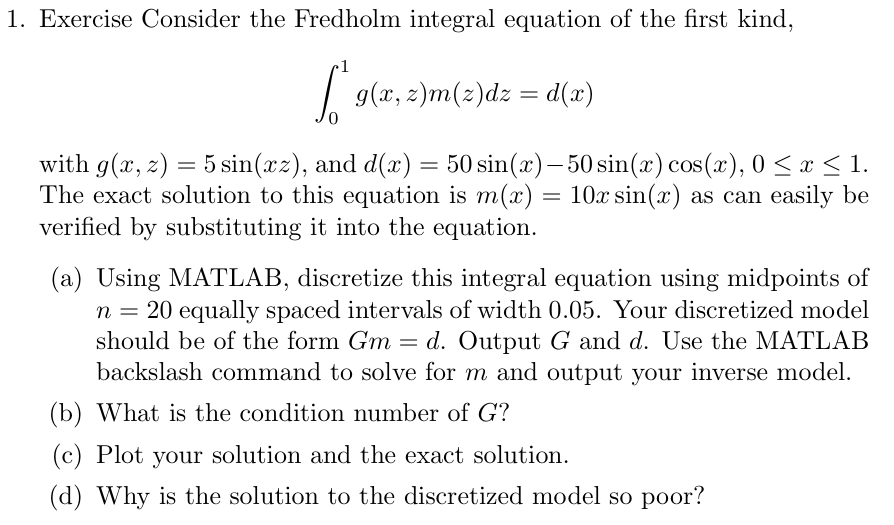
\includegraphics[width=0.8\textwidth]{./images/problem_1_statement.png}
\end{figure}

\subsection*{Solution}

First, let's verify the solution of $m(x)$ via substitution. (This helped me understand the problem immensely, so I will include it here for the sake of completeness)

\begin{align*}
	\int_{0}^{1} g(x,z) m(z) dz &= d(x) \\
	\\
	\int_{0}^{1} 5 \sin(xz) m(z) dz &= 50 \sin(x) - 50 \sin(x) \cos(x) \\
	\\
	\int_{0}^{1} 5 \sin(xz) m(z) dz &= \int_{0}^{1} 5 \sin(xz) m(x) dz \\
	\\
	&= \int_{0}^{1} 5 \sin(xz) \left( 10 x \sin(x) \right) dz \\
	\\
	&= 50 x \sin(x) \int_{0}^{1} \sin(xz) dz \\
	\\
	&= - \frac{50 x \sin(x)}{x} \left[ \cos(xz) \right] |_{0}^{1} \\
	\\
	&= - \frac{50 x \sin(x)}{x} \left( \cos(x) - \cos(0) \right) \\
	\\
	&= 50 \sin(x) \left( 1 - \cos(x) \right) \\
	\\
	&= 50 \sin(x) - 50 \sin(x) \cos(x) = d(x) \,\,\,\, \textcolor{green}{\checkmark}
\end{align*}
	
\subsubsection*{Part A}

Now, suppose that I do not know $m(x)$ for the purposes of this question. Discretizing the given integral using 20 midpoints such that the index $j$ is a member of the set $\{j \in \Z : 1 \leq j \leq 20\}$. Approximating the given Fredholm integral equation of the first kind leads to

\begin{align*}
	\int_{0}^{1} g(x,z) m(z) dz &= d(x) \\
	\\
	\int_{0}^{1} 5 \sin(xz) m(z) dz &\approx \sum_{j = 1}^{20} 5 \sin(xz_{j}) m(z_{j}) \Delta z \\
	\\
	&\approx 5 \sin(xz_{1}) m(z_{1}) \Delta z + 5 \sin(xz_{2}) m(z_{2}) \Delta z + \cdots + 5 \sin(xz_{20}) m(z_{20}) \Delta z
\end{align*}

To fit this discrete numerical integration to the form $G\bv{m} = \bv{d}$, let the variable $x$ be sampled at 20 equally spaced such that the index $i$ is a member of set $\{x \in \Z : 1 \leq i \leq 20\}$. (Note: A bold symbol indicates a vector quantity) This above summation can be expressed as a linear system of equations such that

\begin{align*}
	\begin{bmatrix}
		g_{1,1} & g_{1,2} & \cdots & g_{1,20} \\ 
		g_{2,1} & g_{2,2} & \cdots & g_{2,20} \\ 
		\vdots & \vdots & \ddots & \vdots \\
		g_{20,1} & g_{20,2} & \cdots & g_{20,20}
	\end{bmatrix}
	\begin{bmatrix}
		m(z_{1}) \\ m_(z_{2}) \\ \vdots \\ m(z_{20})
	\end{bmatrix}
	= \begin{bmatrix}
		d(x_{1}) \\ d(x_{2}) \\ \vdots \\ d(x_{20})
	\end{bmatrix}
\end{align*}

where,

\begin{align*}
	G \in \R^{20 \times 20} &: g_{i,j} = 5 \sin(x_i z_j) \Delta z \\
	\\
	\bv{d} \in \R^{20} &: d_i = 50 \sin(x_i) - 50 \sin(x_i) \cos(x_i)
\end{align*}

The vector $\bv{m} \in \R^{20}$ can be solved as

\begin{align*}
	\bv{m} = G^{-1} \bv{d}
\end{align*}

Constructing these vectors and matrices in \MATLAB (provided in file \texttt{prob1.m}), this results in the following quantities for $G$ and $\bv{m}$.






	
	

\end{document}


%----------------------------------------------------------------------
% Additional Copy-and-Paste Templates

% Figure

%\begin{figure}[h] \label{fig: my figure}
%	\centering
%	\includegraphics[width=0.8\textwidth]{./images/<image.png>}
%	\caption{\textcolor{red}{provide a caption}}
%\end{figure}


% Table

%\begin{center}
%	\begin{tabular} { | h1 | h2 | h3 | } \label{tab: my table}
%		
%		\hline
%		x11 & x12 & x13 \\
%		\hline
%		x21 & x22 & x23 \\
%		\hline
%		x31 & x32 & x33 \\
%		\hline
%		
%	\end{tabular}
%	\caption{\textcolor{red}{put caption here}
%\end{center}








